% !TeX encoding = UTF-8
% !TeX spellcheck = en_US
% !TeX root = ../../Thesis.tex
\chapter{Electron beam setup}
\label{ch:Electron beam setup}

\section{Charatarization of a working CRT}
\label{sec:Charatarization of a working CRT}

HAMEG HM507 oscilloscopes \autocite{HM507-manual} were used for testing purposes which contain a D14-363GY/123\autocite{D14363GY123-manual} CRT. Although it only has a bandwidth of \SIrange{0}{50}{\mega\hertz}, which is not sufficient to reach the hyperfine splitting frequency of \SI{461.7}{\mega\hertz} for $^{39}\mathrm{K}$\cite{tiecke:potassium-properties} (or \SI{254}{\mega\hertz} for $^{41}\mathrm{K}$), it was used nevertheless because of its simple construction and availability. The back pin arrangement is shown in \cref{fig:pin arrangement}.

The voltages and currents of the necessary pins to drive the CRT were measured using a \SI{2.5}{\kilo\volt} probe with a voltage divider of 100:1 and are summarized in \cref{tab:D14-363GY/123 tube pin measurements}. It was not possible to measure pin g3 directly. Therefore a HVPS (\cref{sec:HVPS}) was used to set a voltage and the beam diameter was observed. The best focus was achieved with the value written in the table. The voltage offset of x-, and y-plates was not possible to measure directly, since it varies with time to draw the necessary image on the phosphor screen. The given values are the mean of the minimum and maximum measured voltage. The deflection coefficient is summarized in \cref{tab:D14-363GY/123 deflection coefficient}.

\begin{figure}[ht]
	\centering
	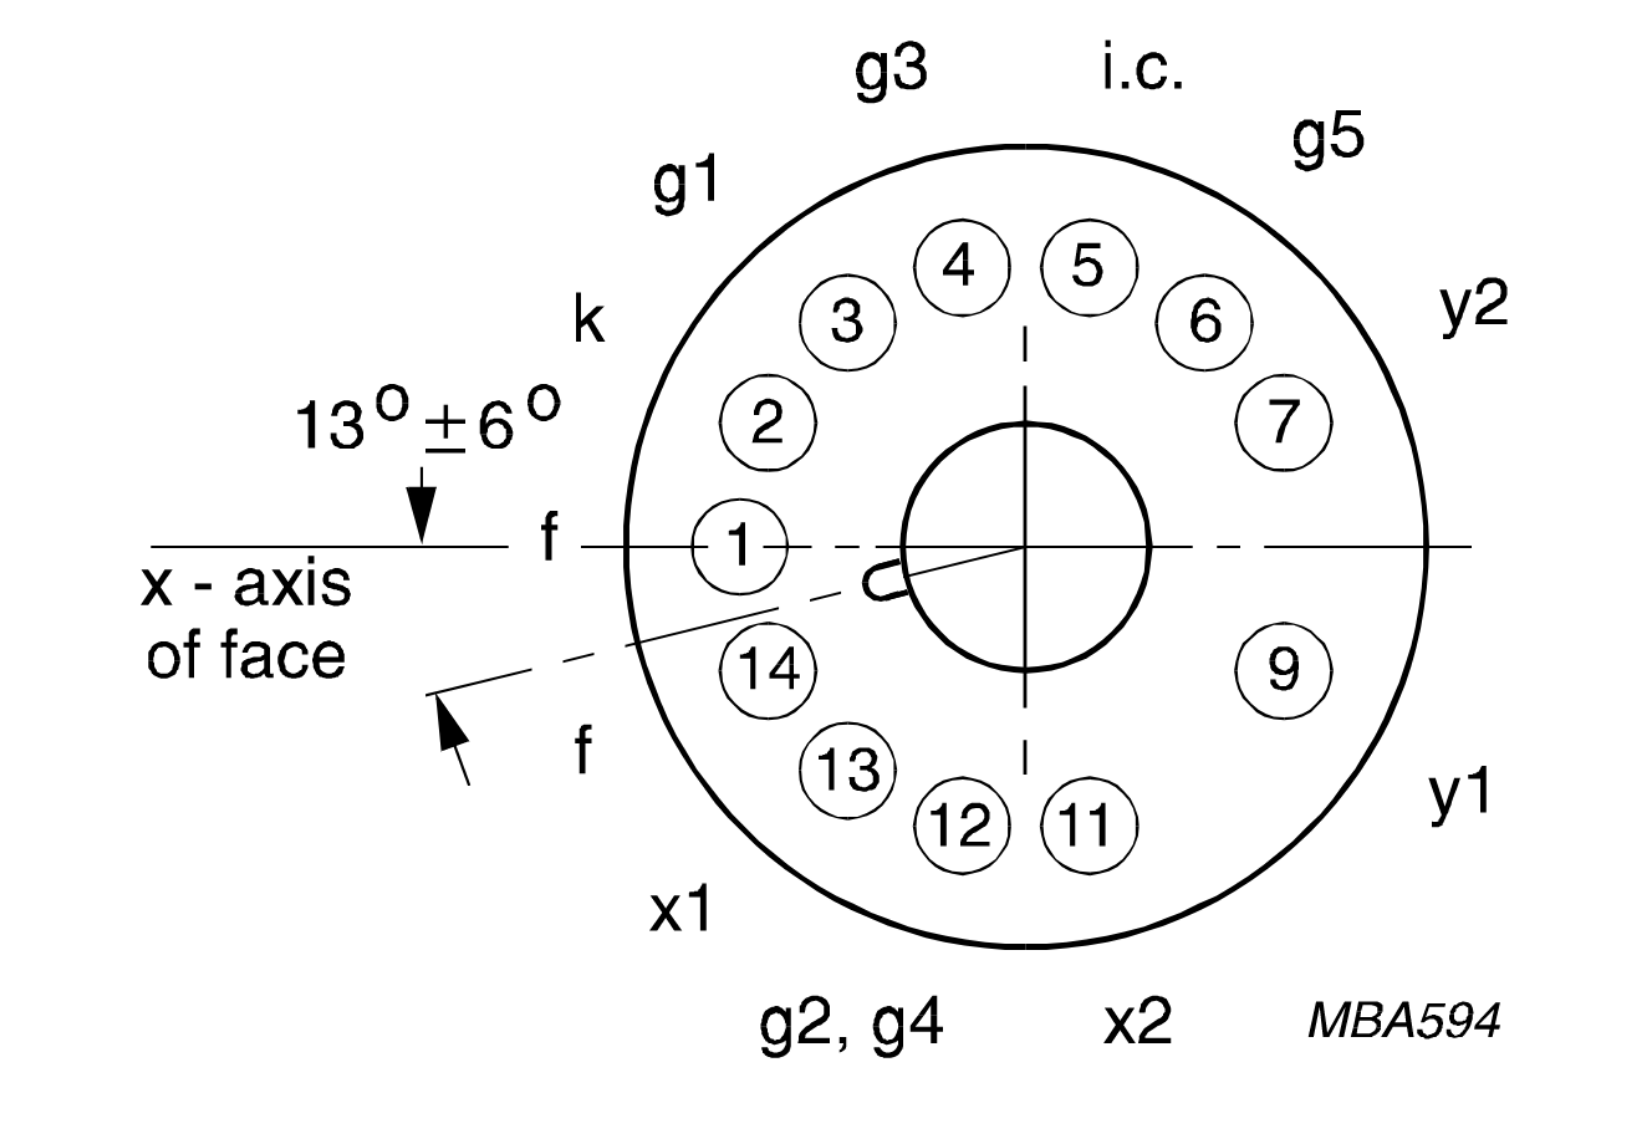
\includegraphics[width=5cm]{./Chapters/e-beam-setup/pin arrangement}
	\caption{Pin arrangement, bottom view from \autocite{D14363GY123-manual}}
	\label{fig:pin arrangement}
\end{figure}


\begin{table}[ht]
	\centering
	\caption{D14-363GY/123 CRT pin measurements}
	\label{tab:D14-363GY/123 tube pin measurements}
	\begin{tabular}{S r *{2}{S}}
		\toprule
		{number} & pin    & {voltage/\si{\volt}} & {current/\si{\micro\ampere}} \\
		\midrule
		1      & f      & -1.99e3              & 86.6e3 \\
		2      & k      & -2.00e3              & -7.6 \\
		3      & g1     & -2.03e3              & 0 \\
		4      & g3     & -1.813e3             & 0 \\
		5      & i.c.   & 71.7                 & 0.1 \\
		6      & g5     & 64.                  & 7.2 \\
		7      & y2     & 78                   & {-} \\
		9      & y1     & 78                   & {-} \\
		11     & x2     & 96                   & {-} \\
		12     & g2, g4 & 71.0                 & 0 \\
		13     & x1     & 96                   & {-} \\
		14     & f      & -1.97e3              & -86.2e3 \\
		\bottomrule
	\end{tabular}
\end{table}

\begin{table}[ht]
	\centering
	\caption{D14-363GY/123 deflection coefficient from \autocite{D14363GY123-manual}}
	\label{tab:D14-363GY/123 deflection coefficient}
	
	\begin{tabular}{*{2}{l} l}
		\toprule
		horizontal & $M_x$ & \SI{19}{\volt/\centi\meter} \\
		vertical   & $M_y$ & \SI{11.5}{\volt/\centi\meter} \\
		\bottomrule
	\end{tabular}
\end{table}


\section{High Voltage Power Supply HVPS}
\label{sec:HVPS}

To produce high dc voltages to drive the CRT, four HCP 14-6500 power supplies \autocite{fug-hcp-manual} were used. They were named `HVPS 1' to `HVPS 4' and can provide up to \SI{2}{\milli\ampere} at \SI{\pm 6.5}{\kilo\volt}. To connect the output to the CRT pins, BNC cables were refitted with a save high voltage (SHV) connector on one side while on the other end the BNC connector was kept (\cref{fig:Coaxial cable with SHV and BNC connector}). A \SI{6}{\kilo\volt} probe was used to obtain the breakdown voltage, which is around \SI{3}{\kilo\volt} caused by the coaxial cable which was not built do sustain high voltages.

\begin{figure}[ht]
	\centering
	
	\missingfigure[figwidth=0.9\textwidth]{Figure of SHV \& BNC connector cable.}
	
	\caption{Coaxial cable with SHV and BNC connector.}
	\label{fig:Coaxial cable with SHV and BNC connector}
\end{figure}

\subsection{Ripple measurement}
\label{subsec:ripple measurement}
Each power supply was measured for its ripple with a set voltage of \SI{2}{\kilo\volt}. A \SI{2.5}{\kilo\volt} probe (attenuation ratio 100:1) was connected to an oscilloscope set to ac coupling with a timescale of \SI{1}{\milli\second}. To get the electronic noise of the oscilloscope itself, the probe was shorted and the noise measured. A picture of a measurement is shown in \cref{fig:measurement HVPS ripple} with the values summarized in \cref{tab:measurement HVPS ripple}. As can be seen, the ripple is very close to the noise level and can not really be distinguished.

\begin{figure}[ht]
	\centering
	
	\includegraphics[width=0.9\textwidth]{./Chapters/e-beam-setup/ripple HVPS1}

	\caption{Measurement of HVPS ripple.}
	\label{fig:measurement HVPS ripple}
\end{figure}

\begin{table}[ht]
	\centering
	\caption{HVPS ripple}
	\label{tab:measurement HVPS ripple}
	\begin{tabular}{l S}
		\toprule
		device & {ripple/\si{\milli\volt}} \\
		\midrule
		short  & 116 \\
		HVPS 1 & 136 \\
		HVPS 2 & 138 \\
		HVPS 3 & 194 \\
		HVPS 4 & 204 \\
		\bottomrule
	\end{tabular}
\end{table}

\section{CRT wiring}\label{sec:CRT wiring}
A schematic of the supplied power is shown in \cref{fig:schematics of wiring}. The pin i.c. stands for internally connected and is wired to pin g2, g4. A small ac or dc voltage is necessary to drive the heater filament f. This part of the setup is explained in \cref{sec:Heater}.


\begin{figure}[H]
	\centering
	
	\begin{circuitikz}[european]
		% !TeX encoding = UTF-8
% !TeX spellcheck = en_US
% !TeX root = ../../Thesis.tex


%\draw [help lines] (0,0) grid (10,10);
		
\newcommand{\hvps}[2] % corordinates of bottom left corner, label
% draw a hvps
{		
	% draw HVPS
	\draw (0 + {#1}[0], 0 + {#1}[1]) rectangle (2.5 + {#1}[0], 2.5 + {#1}[1]); % box of size 2.5
	\node[above] at (1.25 + {#1}[0], 2.5 + {#1}[1]) {#2};	% label for box
	\draw (3 + {#1}[0], 1 + {#1}[1]) -- (1.5 + {#1}[0], 1 + {#1}[1]) to[vsource] (1.5 + {#1}[0], 2 + {#1}[1]) -- (3 + {#1}[0], 2 + {#1}[1]);  % voltage supply
	\draw (1.5 + {#1}[0], 0.5 + {#1}[1]) -- (3 + {#1}[0], 0.5 + {#1}[1]) node[ground] {}; % ground
}

\newcommand{\coaxial}[2] % coordinates of left inner wire, length of cable
% draw a coaxial cable with given length
{
	\draw (0 + {#1}[0], {#1}[1]) to[short, *-*] (#2 + {#1}[0], {#1}[1]); % middle line
	\draw (1 + {#1}[0], {#1}[1]) circle [radius=0.5]; % left circle
	\draw (#2 - 1 + {#1}[0], {#1}[1]) circle [radius=0.5]; % right circle
	\draw (1 + {#1}[0], 0.5 + {#1}[1]) -- (#2 - 1 + {#1}[0], 0.5 + {#1}[1]); % top line
	\draw (0 + {#1}[0], -0.5 + {#1}[1]) to[short, *-*] (#2 + {#1}[0], -0.5 + {#1}[1]); % bottom line
}

% HVPS 4
\hvps{(0, 0)}{HVPS 4}
\draw (3, 2) -- (3, 1.5);
\coaxial{(3, 1.5)}{5}
\draw (8, 1.5) -- (10, 1.5);
\node [right] at (10, 1.5) {i.c.};

% HVPS 3
\hvps{(0, 4)}{HVPS 3}
\draw (3, 6) -- (3, 5.5);
\coaxial{(3, 5.5)}{5}
\draw (8, 5.5) -- (10, 5.5);
\node [right] at (10, 5.5) {g3};

% HVPS 2
\hvps{(0, 8)}{HVPS 2}
\draw (3, 10) -- (3, 9.5);
\coaxial{(3, 9.5)}{5}
\draw (8, 9.5) -- (10, 9.5);
\node [right] at (10, 9.5) {f};
\draw (9, 9.5) to[sV, *-] (9, 8); % ac voltage source
\draw (9, 8) to[short, *-] (10, 8);
\node [right] at (10, 8) {f};
\draw (9, 8) -- (9, 7) -- (10, 7);
\node [right] at (10, 7) {k};

% HVPS 1
\hvps{(0, 12)}{HVPS 1}
\draw (3, 14) -- (3, 13.5);
\coaxial{(3, 13.5)}{5}
\draw (8, 13.5) -- (10, 13.5);
\node [right] at (10, 13.5) {g1};
	\end{circuitikz}

	\caption{Schematics of supplying CRT pins with power.}
	\label{fig:schematics of wiring}
\end{figure}


\section{Heater}
\label{sec:Heater}

\begin{figure}[ht]
	\centering
	
	\begin{subfigure}[b]{0.9\textwidth}
		\begin{circuitikz}%[width=0.9\textwidth]
			% !TeX encoding = UTF-8
% !TeX spellcheck = en_US
% !TeX root = ../../Thesis.tex


%\draw [help lines] (0, 0) grid (8, 4);
%\filldraw (0, 0) circle (0.5mm);

% left half with transformer
\draw (0, 0)
to [sV, label = \SI{230}{\volt}] ++ (0, 2)
to [normal open switch]  ++ (2, 0);
\draw (2, 2) node [transformer core, anchor=A1] (transformer) {}
	(transformer.inner dot A1) node[circ]{}
	(transformer.inner dot B1) node[circ]{};
\draw (transformer.A2) -- (0, 0|-transformer.A2) -- (0, 0);

% right half
\ctikzset{european resistors}
\draw (transformer.B1)  to [fuse, label = \SI{200}{\milli\ampere}] (6, 2)
	to [pR, name=pot] ++ (0, -2) -- (6, 0|-transformer.B2);
\draw (transformer.B2) to [ammeter] (6, 0|-transformer.B2);

\draw (6, 3) to [short, -*] (6, 2);
\node [right] at (6, 3) {$V_{\mathrm{bias}}$};

\draw (6, 0|-transformer.B2) to [short, *-] (7, 0|-transformer.B2);
\node [right] at (7, 0|-transformer.B2) {f};

\draw (pot.wiper) -- (7, 1);
\node [right] at (7, 1) {f};
		\end{circuitikz}
		\caption{Circuit diagram of filament power supply.}
	\end{subfigure}
	
	\vspace{1cm}

	\begin{subfigure}[b]{0.9\textwidth}
		\missingfigure[figwidth=\textwidth]{picture of ac bias voltage}
		\caption{Picture of built filament power supply.}
	\end{subfigure}
	
	\caption{AC power supply used to heat the filament with a \SI{-2}{\kilo\volt} bias voltage.}
	\label{fig:heater_circuit}
	\todo[inline]{check if really \SI{14}{\ohm} or if it event exists}
\end{figure}

The heater provides an adjustable ac voltage, which is used to regulate the temperature of the cathode. In the cold state, the heater filament has a an electrical resisitance of approximately \SI{15}{\ohm}, when the filament is hot, this value rises to \SI{90}{\ohm}. The normal heater voltage for the D14-363GY/123 during  operation is \SIrange{6.0}{6.6}{\volt} according to \cite{D14363GY123-manual}. 
Our ac-power supply (shown in figure \ref{fig:heater_circuit}) consists of an isolation transformer (from grid voltage to 12 V), its primary  and secondary circuits are isolated up to \SI{4}{\kilo\volt} \cite{DS44231-DataSheet}. The power supply has two  banana plug sockets to connect to the heater filament. 
It is connected to the transformer in series with a \SI{100}{\ohm} potentiometer. Using the full resistance, there is a voltage of approximately \SI{5.7}{\volt} applied to the heater filament, by lowering the resistance this value can goes up to nearly the full voltage of the transformer. 
The current running through the filament is measured with an integrated ampere meter \cite{ACA-20PC-manual}, that measures currents up to two \SI{2}{\ampere} with \si{\milli\ampere} accuracy.

At the beginning of operation it is recommendable to set the maximum resistance and slowly increase the current to the desired value once the filament is heated up. As the resistance of the cold filament is significantly lower, high onset currents could otherwise damage it.  